\cleardoublepage
\phantomsection
\addcontentsline{toc}{chapter}{Введение}
\chapter*{Введение}
\label{chap:introduction}

В информационных технологиях с течением времени все больше развития получают методы работы с данными, при которой исчерпывающие исходные данные о среде задать невозможно, или нецелесообразно, в связи с противоречивостью или слабой формализацией среды.
Особенностью такого рода подхода является возможность применения в задачах, не предназначенных изначально для обработки компьютером, в которых традиционные алгоритмы, как правило, сильно ограниченны.

Один из подходов к работе с нечеткой логикой ---  искусственные нейронные сети (ИНС), представляет собой математическую модель, построенную по принципу организации и функционирования биологических нейронных сетей, состоящих из нервных клеток.

Понятие ИНС появилось в результате разработки Мак-Каллоком и Питтсом в 1943 году компьютерной модели нейронной сети на основе математических алгоритмов и теории деятельности головного мозга.
Впоследствии, после разработки алгоритмов обучения (в частности, метода обратного распространения ошибки), получаемые модели стали использовать в практических целях: в задачах прогнозирования, для распознавания образов и др.
ИНС представляют собой систему соединённых и взаимодействующих между собой относительно простых (искусственных) нейронов. 
 
Возможность обучения — главное преимущество нейронных сетей перед традиционными алгоритмами. 
Нейронные сети способны в процессе обучения выявлять сложные нелинейные зависимости между входными данными и выходными, а также на основе полученных данных обобщать зависимости на всю область. 

Научно-технический прогресс в информационных технологиях и развитие быстродействия вычислительных машин во многом ответственны за повторный всплеск интереса к нейронным сетям. 
Здесь находят применение данные о функционировании различных подсистем головного мозга (в первую очередь зрительная и слуховая). 
При текущем уровне производительности компьютеров на них возможна работа искусственных нейронных сетей, выполняющих ранее недоступные для компьютера задачи (вождение автомобиля, победа в 2017 году машины над человеком в игре \en{Go}).
Это открывает новые возможности взаимодействия с информацией и качественно новый уровень возможностей ее использования.

ИНС нашли применение в системах: поисковых, 
машинного перевода, распознавания лиц, эмоций, объектов, и т.д.

Проекты \en{Blue Brain Project} и \en{Human Brain Project} нацелены на создание инфраструктуры для моделирования всего мозга целиком в изолированной компьютерной среде, создание цифровых реконструкций мозга грызуна и, в конечном счете, человека. 
Некоторые коллективы исследователей заняты исследованием технической реализуемости симуляции. 
Так, в Японии, на суперкомпьютере K, (занимает 7-ю позицию в рейтинге \en{Top-500} по состоянию на ноябрь 2016) в 2017 году была предпринята тестовая попытка воссоздания нейронной сети, приближенной к биологическому мозгу человека. 
\en{(Largest neuronal network simulation achieved using K computer.)}
В результате удалось запустить на фреймворке \en{NEST} ~\cite{nest} цифровой аналог 1\% объема мозга, на основании чего группа ученых из \en{RIKEN HPCI} делают предположение, что с появлением экзафлопсного суперкомпьютера станет возможной симуляция всего мозга человека.

Данная работа выполнена в рамках проекта искусственной когнитивной архитектуры для интеллектуальных систем --- нейромодулирующей когнитивной архитектуры (\en{NEUCOGAR}~\cite{neucogar}).
Модель биомиметически вдохновлена и адаптирует роль нейромодуляторов человеческого мозга в вычислительные среды.
Основной идеей работы является моделирование ответственных за моторный вывод в контексте эмоциональной оценки областей мозга.
Задачами работы являются:
\begin{itemize}
	\item выделение важных для моторной активности участков мозга
	\item построение нейронной сети, повторяющей биологическое устройство моторного вывода мозга
	\item интеграция когнитивной архитектуры \en{NEUCOGAR} с полученной моделью
\end{itemize}

Моделирование проводилось во фреймворке \en{NEST}, в качестве языка программирования применяется \en{Python}.




\begin{comment}
Это --- пример оформления выпускной квалификационной работы в \LaTeX.
Набирая текст в этой системе, не нужно задумываться об оформлении документа по ГОСТу.

Обычный текст вводится так, как есть.
Отдельные предложения имеет смысл отделять друг от друга новыми строками: это помогает в редактировании, но не обязательно.

Абзацы отделяются друг от одной или более пустыми строками.
Каждый абзац должен содержать единственную, законченную мысль.

Команды, начинающиеся с символа \verb|\|, являются специальными инструкциями \TeX{} или \LaTeX.
Чтобы оставить пробел после команды, нужно поставить фигурные скобки: \verb|\TeX{}|.

Помимо команд, также существуют окружения, использующиеся для больших блоков содержимого:
\begin{verbatim}
\begin{environment}
content
\end{environment}
\end{verbatim}

Внешние кавычки печатаются <<так>>.
Внутренние кавычки ставятся ,,так``.
Также можно использовать команду \verb|\enquote| \enquote{для автоматического \enquote{определения} уровня вложенности}.

Есть 3 основных типа тире.
Дефис \verb|-| используется для разделения сложных слов и некоторых предлогов: квадратно-гнездовой.
Короткое тире \verb|--| \en{(en-dash)} встречается в числовых диапазонах: 1970--2015.
Длинное тире \verb|---| \en{(em-dash)} --- это обычное тире в предложениях.

Для набора английского текста используйте команду \verb|\en| или окружение \verb|english|.

В данном классе и шаблоне уже настроено практически всё, что может понадобиться при написании работы.

Рисунки включаются так:
\begin{verbatim}
\begin{figure}
\centering
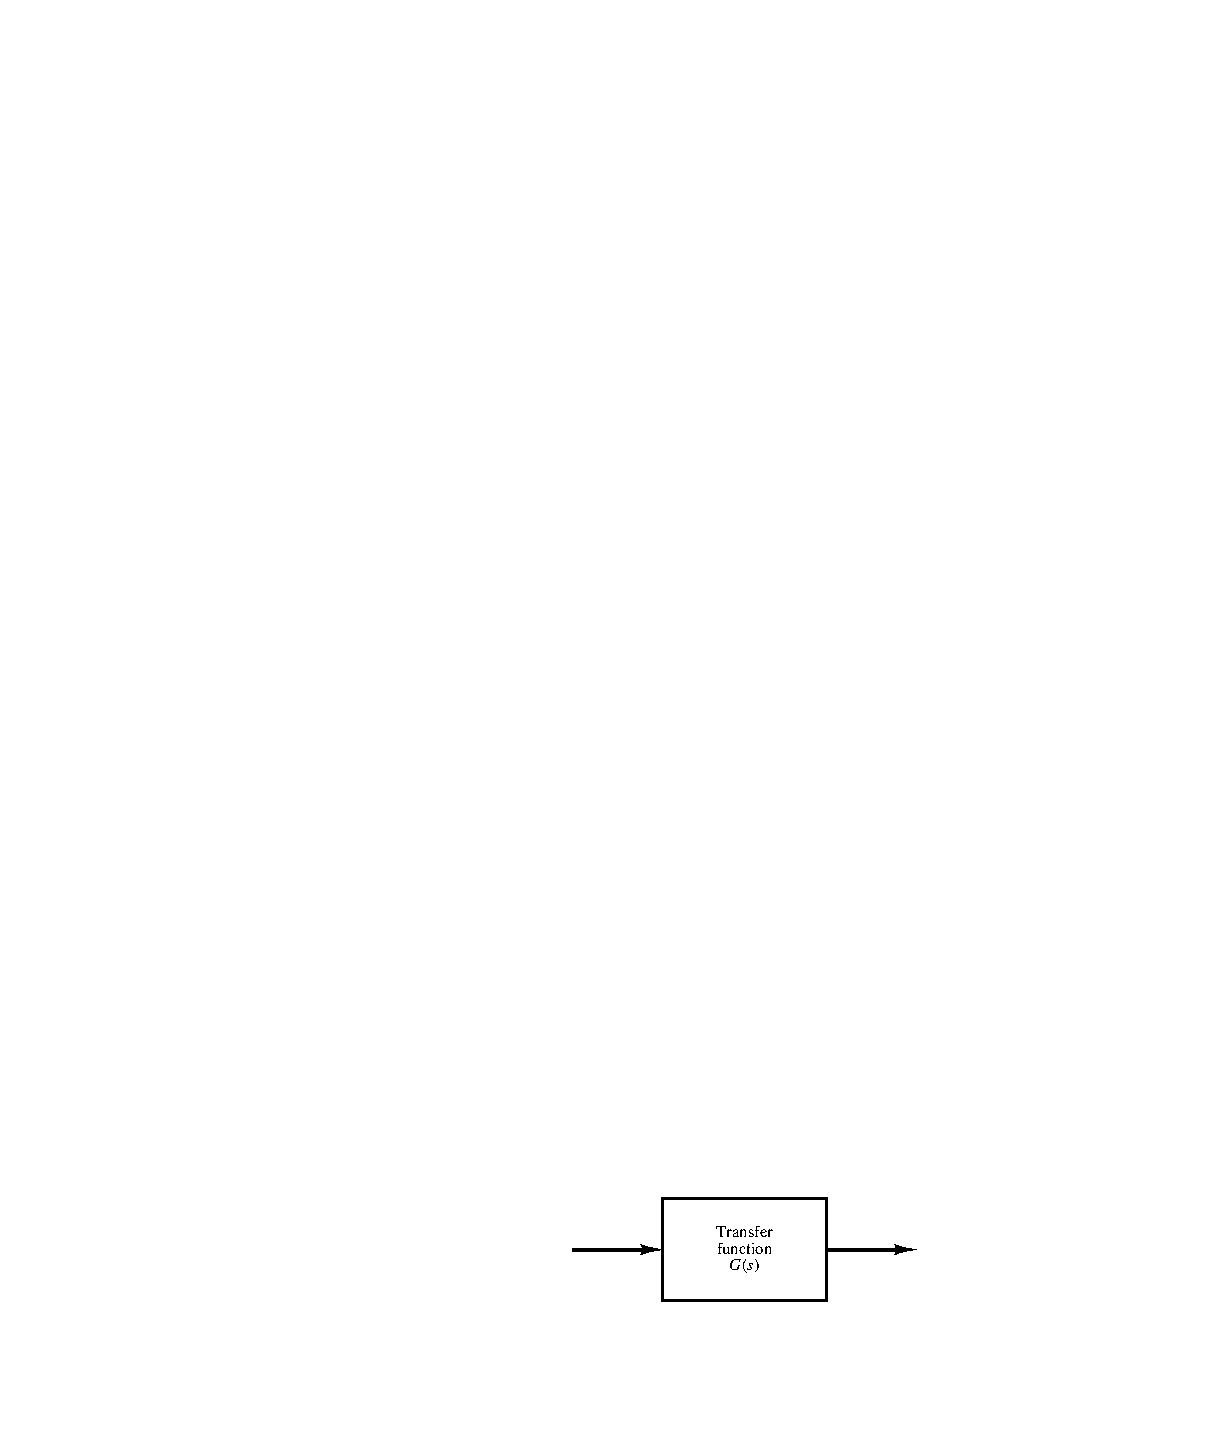
\includegraphics[width=\linewidth]{sample_figure}
\caption{Пример рисунка}
\label{fig:sample_figure}
\end{figure}
\end{verbatim}

\begin{figure}
\centering
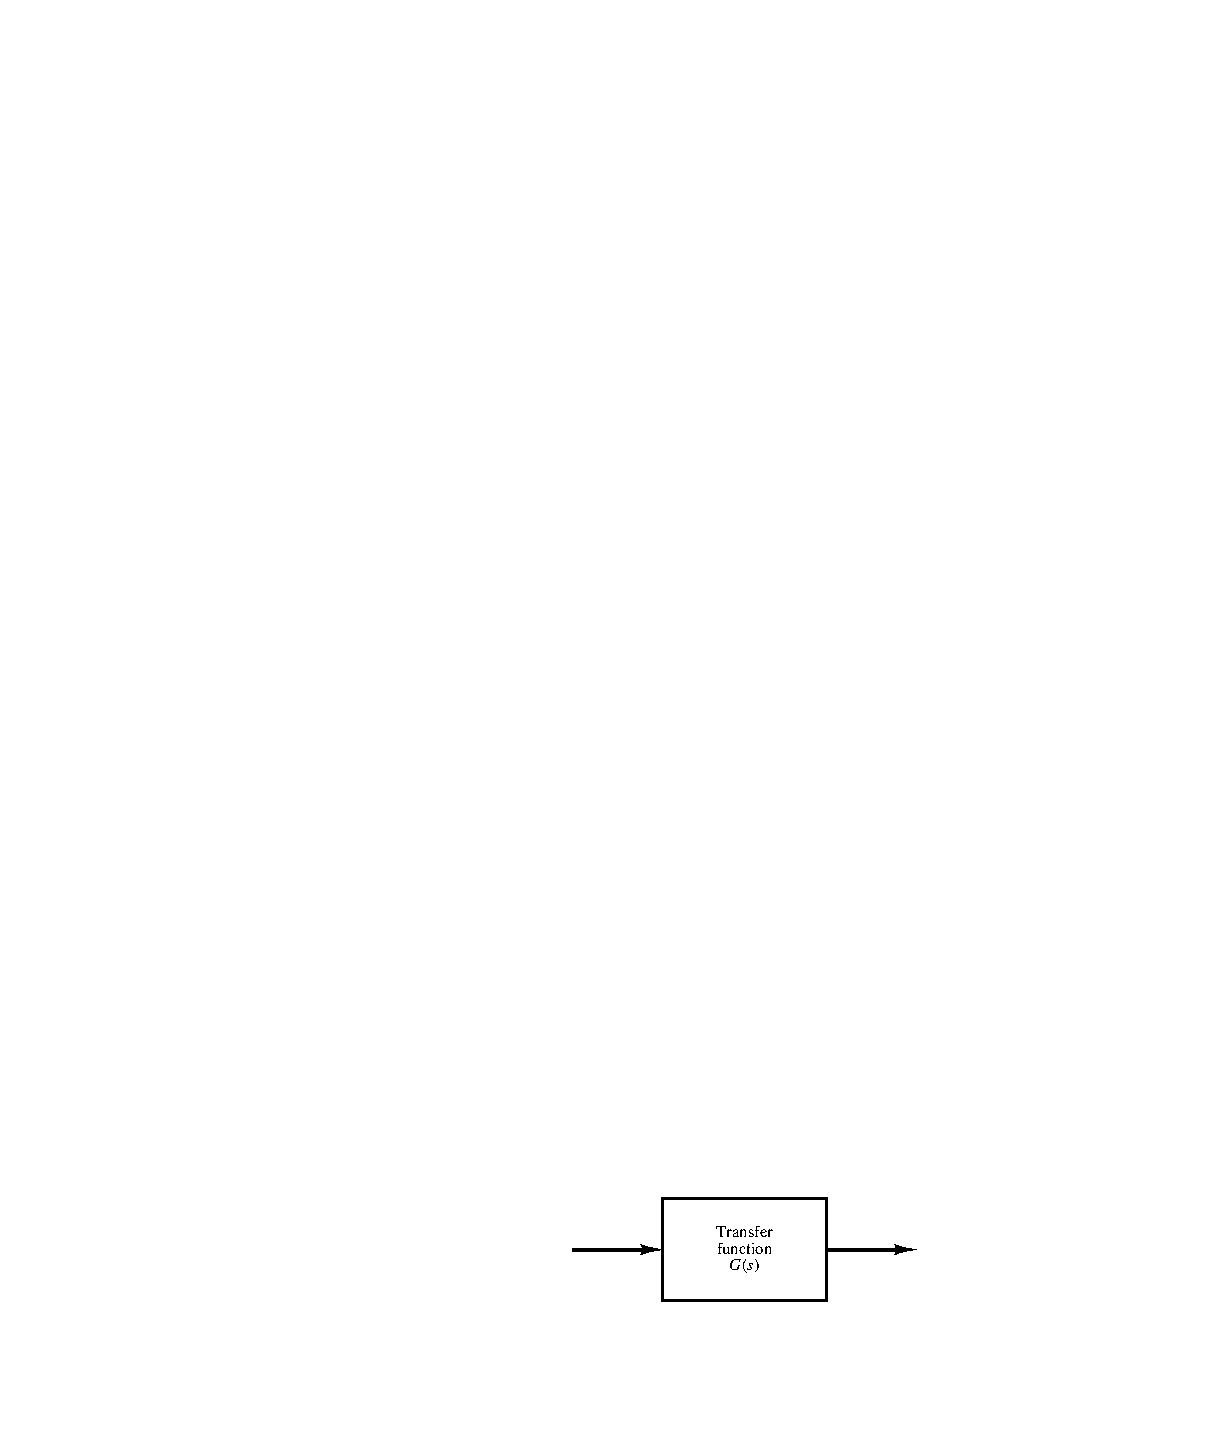
\includegraphics[width=\linewidth]{sample_figure}
\caption{Пример рисунка}
\label{fig:sample_figure}
\end{figure}

Таблицы верстаются так:
\begin{verbatim}
\begin{table}
\caption{Пример таблицы}
\label{tab:example_table}
\begin{tabular}{l c r}
\toprule
Заголовок 1 & Заголовок 2 & Заголовок 3 \\
\midrule
11 & 12 & 13 \\
21 & 22 & 23 \\
31 & 32 & 33 \\
\bottomrule
\end{tabular}
\end{table}
\end{verbatim}

\begin{table}
\caption{Пример таблицы}
\label{tab:example_table}
\begin{tabular}{l c r}
\toprule
Заголовок 1 & Заголовок 2 & Заголовок 3 \\
\midrule
11 & 12 & 13 \\
21 & 22 & 23 \\
31 & 32 & 33 \\
\bottomrule
\end{tabular}
\end{table}

Ссылаться на рисунки и таблицы можно командой \verb|\ref|: рис.~\ref{fig:sample_figure} и табл.~\ref{tab:example_table}.

Ссылки на источники создаются командой \verb||: хороший обзор возможностей \LaTeX{} можно найти в~\cite{oetiker1995not}.
\end{comment}

